\documentclass[12pt, oneside, a4paper]{article}
\usepackage{ifpdf}
\usepackage{graphicx}
\usepackage[colorlinks,bookmarksopen,linkcolor=black,pdfauthor={Sharad,Prabhakar,Vikram},urlcolor=blue]{hyperref}
\usepackage[colorlinks,bookmarksopen]{hyperref}
\begin{document}
\begin{center}
\textbf{VISVESWARAYA TECHNOLOGICAL UNIVERSITY}
\end{center}
\begin{center}
\textbf{BELGAUM}\\
\thispagestyle{empty}
\begin{figure}[htb]
\begin{center}
\ifpdf
	
\includegraphics[scale=0.50]{vtu.png}
\else
%	
\includegraphics[scale=0.50]{vtu.png}
\fi
\end{center}
\end{figure}
\textbf{SRI JAYACHAMARAJENDRA COLLEGE OF ENGINEERING}
\textbf{MYSORE-570006}\\
\textsc{department of computer science and engineering}
\end{center}
\begin{figure}[htb]
\begin{center}
\ifpdf

\includegraphics[scale=0.30]{./logo.png}
\else
%	
\includegraphics[scale=0.30]{/home/prabhakar/logo.odg}
\fi
\end{center}
\end{figure}
\begin{center}
\textbf{\underline{Project on}}\\
\textsc{IMPLEMENTATION OF HANDWRITTEN LEXER AND PARSER FOR $\beta$parse - A 'C' SUBSET\\}
\emph{\\Guidance of}\\
\textbf{P.M. SHIVMURTHY}\\
\textit{Lecturer}\\
\textit{Department of CS$\&$E, SJCE, Mysore.}\\
\end{center}
Team:
\begin{center}
\begin{tabular}{|c|c|c|}
\hline
%% row 1
\textsc{name}
&\textsc{roll no}
&\textsc{usn}
\\\hline
%% row 2
\textsc{vikram tv}
&61
&\textsc{4jc07cs120}
\\\hline
%% row 3
\textsc{prabhakar gouda}
&37
&\textsc{4jc07cs070}
\\\hline
%% row 4
\textsc{sharad d}
&03
&\textsc{4jc06cs089}
\\\hline
\end{tabular}
\end{center}
\newpage
\thispagestyle{empty}
\tableofcontents
\newpage
\pagenumbering{arabic}

\section{Overview}
$\beta$ - parse language is the beta version of parsing of our own language.  It involves the best possibilities that we have seen from the classic language `C'.  Our language is purely a subset of the higher level language - 'C'.  It takes program written as per the rules and syntax of our language as input and validates the syntax of the program.  In case of any error in the program it display the line number in which the error is detected and possible type of error.  It also generates a parse tree for the user convenience.  This implementation is done in two phases - the lexical phase and the parsing phase.\\

\section{Glossary}
\begin{tabular}{ll}
%% row 1
$\beta$parse & Our own defined language.\\
source program & User program written in $\beta$parse spec.\\
keywords & The keywords supported by our language.\\
HTML & Hyper Text Markup Language.\\
dotty & Product to support graph display.\\
kgraphviewer & Product to support graph display (kde version).\\
**.cs & (C Subset) Our own language extension\\ & although any extension is supported.\\
delimiter & any character other than in the range a-z A-Z 0-9.\\
whitespace & a space, a tab or a newline is a whitespace.\\
Lexeme & A sequence of characters in the source program that matches\\ 
& the pattern for a token.\\ 
Token & A pair consisting of a token name and an optional attribute value.\\
Pattern & A description of the form that the lexemes of a token may take.\\
Symbol Table & The data structures that are used by parser and lexer\\ 
& to hold information.\\
Lexer & Scanner which finds the token and return to the parser.\\
Parser & Which handles the token.\\
\end{tabular}

\section{Constructs of the Language}
The program consists of 2 parts:
\begin{itemize}
\item The `file inclusion' part
\item The `function definition' part
\end{itemize}
\subsection{File Inclusion}
File inclusion is done using the keyword \textbf{include}.\\

\hspace{.5in} \textbf{Syntax:}
	
\hspace{1in}  \textbf{include} \emph{$"$file name$"$}\\


File names should not contain any extensions.  Hence unique files are included.
The include directive can be placed anywhere in the program and every file that is to be included should in a separate line.\\

\emph{Example}: include $"$stdio$"$\\\\
The directive includes the file $"$stdio$"$ to the current scope.


\subsection{Function}
Function can be started by specifying the function name and parameter list for the function enclosed within parenthesis.  Every function starts with the special character $'$\{$'$ and ends with $'$\}$'$.The function definition is very similar to $'$C$'$\\

\hspace{.5in} \textbf{Syntax:}
	
\hspace{1in}  functionName (parameterList)\\

\hspace{1in}\{\\

\hspace{1in}$\cdots$\\

\hspace{1in}\emph{body}\\

\hspace{1in}$\cdots$\\

\hspace{1in}\}\\
The parameter list can be zero or more.  The elements of the list should be separated by comma (,).  The function body can contain any number of basic statements like assignment, increment, decrement that resemble the 'C' statements.  The body can also include the relational operations, looping operations and function calls also.\\

\emph{Example}: main(int argc, char **argv)\{ s = p + v; a++; \}\\

\hspace{1in} or\\

\hspace{.75in}main(int argc, char  **argv)

\hspace{.75in} \{

\hspace{1in}s = p + v;

\hspace{1in}a++;

\hspace{1.15in} $\dots$

\hspace{.75in}\}

Every statement with in the function body should end with a semicolon (;) similar to `C' language syntax.
The \emph{return value} of the function lies in its name only.\\

The details of the various types of statements in our language construction is dealt in the next section.

\section{Syntax of Statements}
The following are the various types of syntax that are used:

\subsection{Operators and Symbols}
The following \textbf{operators} are supported in the language.  It includes the basic arithmetic operators.\\
\begin{tabular}{ll}
+ & to perform binary addition of two variables.\\
- & to perform binary subtraction of two variables.\\
$*$ & to perform binary multiplication of two variables.\\
/ & to perform binary division of two variables.\\
, & (comma) to separate the variable declarations and also to\\ &  separate assignment statements.\\
= & to assign the rvalue obtained by an expression to the lvalue.\\
$\wedge$ & to perform the binary power operation.\\
\end{tabular}
\\\\\textbf{Relational Operators:}\\
The following operators on two variables or expressions returns a Boolean value.  These operators are used to test the various conditions in the language.\\\\
\begin{tabular}{|l|l|c|}
\hline
%% row 1
Operator
&Operation
&Notation
\\\hline
%% row 2
== 
&checks for equivalence of two variables or expressions.
&EE
\\\hline
%% row 3
!= 
&checks if left variable or expression is equal to or not to the right.
&NE
\\\hline
%% row 4
$>$  
&checks if left variable or expression is greater than to the right.
&GT
\\\hline
%% row 5
$<$ 
&checks if left variable or expression is less than or equal to the right.
&LT
\\\hline
%% row 6
$>$= 
&checks if left variable or expression is greater than or equal to the right.
&GE
\\\hline
%% row 7
$<$=  
&checks if left variable or expression is less than or equal to the right.
&LE
\\\hline
\end{tabular}
\\\\The following \textbf{symbols} are used:\\\\
\begin{tabular}{ll}
; & to terminate a statement in the program.\\
( ) & to specify a function call and the precedence of evaluation.\\
\{ &to open the block statement.\\
\} & to close the block statement.\\
\end{tabular}

\subsection{Variables}
The language supports all the characters (both uppercase and lowercase) of the English Language.  It also supports the integer values.  Any variable can be declared on the lines of variable declaration in 'C'.
\begin{itemize}
\item The variable can have both the characters and integers in it.
\item The variable should start with an English character and not by an integer.
\item The variable can be of any length.
\item Keywords of the language cannot be used as variables.
\end{itemize}

\subsection{Commenting}
Commenting in the language is similar to the commenting styles in C language.

\hspace{.5in} \textbf{Syntax:}
	
\hspace{1in}  /*\emph{comment} */\\

Everything between $/*$ and $*/$ also considered as comment it is not parsed.

\subsection{Declaration}
The type declaration of variables used in the program are not needed and the variables can be used directly, although some of the basic data types (integer, float, character) are provided.  The variable is casted according to the rvalue used in the program.  Also multiple declaration of variables in a single line separated by commas are possible.  The declarations are to be terminated by a semicolon to mark the end.\\

\begin{tabular}{|c|c|l|}
\hline
%% row 1
Keyword
&Meaning
&Example statement
\\\hline
%% row 2
int
&Integer
&int a,b;
\\\hline
%% row 3
float
&Floating point
&float fl;
\\\hline
%% row 4
char
&character
&char ch;
\\\hline
\end{tabular}

The declaration of a new variable is made at its first assignment.

\emph{Example}: a = 3;\\\\
This declares the variable 'a' and assigns to it the value 3.

\subsection{Assignment}
The assignment statements are implemented based on the syntax of assignments done in 'C' Language.  The `rvalue' is assigned to the `lvalue'.  The left value can consist only one variable and not a number as a single value cannot be assigned to two or more variables on left.  The right value can consist of a variable, number or a combination of both to form a compound expression.\\

All assignment statements should terminate with a semicolon.\\

The following assignment statements are supported:\\
\begin{itemize}
\item Direct Assignment as `a = b;'
\item Evaluation of expressions within `( )', that has the highest order.
\end{itemize}

\subsection{Relational Condition Checking - The `\textit{if-else}' construct}
The language uses the following syntax to perform the relational condition checking.

\hspace{.25in} \textbf{Simple IF syntax:}

\hspace{.5in}  \textbf{if}(\textit{condition})\\

\hspace{.5in} \{\\

\hspace{1in}statements\\

\hspace{.5in}\}\\


\hspace{.25in} \textbf{IF-ELSE syntax:}

\hspace{.5in}  \textbf{if}(\textit{condition})\\

\hspace{.5in} \{\\

\hspace{1in}statement1\\

\hspace{.5in}\}\\

\hspace{.5in} \textbf{else}\\

\hspace{.5in}\{\\

\hspace{1in}statement2\\

\hspace{.5in}\}\\


The \emph{if} keyword tests for the Boolean value of the condition.  The condition uses the relational operators between two variables or expressions.  If the condition is true, then the \emph{statements1} are executed.  In the second case, if the condition results false then the keyword \emph{else} is parsed to execute the \emph{statements2}.\\

The statements1 and statements2 can inturn contain any number of nested `\textit{if-else}' conditions.

\subsection{Looping Construct}
The looping construct is implement in the language using the keywords \textbf{for} and.\\

\hspace{.25in} \textbf{Syntax:}

\hspace{.5in}  \textbf{for}(\emph{initialization};\emph{condition};\emph{incrementation};)

\hspace{.5in}\{\\

\hspace{.5in} statements\\

\hspace{.5in}\}\\


Looping of the \emph{statements} is done only if the \emph{condition} is satisfied.\\
\textit{Example}

\hspace{.5in}\textbf{for}(i = 0 ; i$<=$ n ; i = i + 1;)

\hspace{.5in}\{\\

\hspace{1in} $\dots$

\hspace{1in} a = a + b;

\hspace{1in} $\dots$

\hspace{.5in}\}

The statements can in turn contain any number of nested looping structures.

\subsection{Nesting of Statements}
The language supports nesting of statements.

The statements containing the `\textit{if-else}' and `\textit{for-loop}' can be nested.  Any number of statements can be used in them.  Also the nested can be to any level in depth.  The `if' can nest `if' or `loop' or both.  Similarly, `loop' can nest `loop' or `if' or both.

Thus any of the \emph{nesting} combinations works well with the language.

\subsection{Program}
The language supports to have \emph{any number of} `functions', `file inclusions', `conditional executions', `looping constructs' and `statements' in the program.  Each construct is supposed to be terminated by appropriate terminator.
\section{Transition Diagrams}
\paragraph{}

Transition diagram has collection of nodes called as states. Each state represents a condition that could occur during the process of scanning the input looking for a lexeme that one of the several patterns.
\subsection{Transition diagram for relational operators}

\paragraph{}

The transition starts from state 0(initial state). After scanning the symbol $<$(less then) it goes to state '1' there are three options from state '1' namely 2, 3 and 4 shown in diagram, where state 2, 3 and 4 are final states which returns respective tokens. Similar operation in other states, it is clear in below diagram.\\
\begin{figure}[htb]
\begin{center}
\ifpdf
	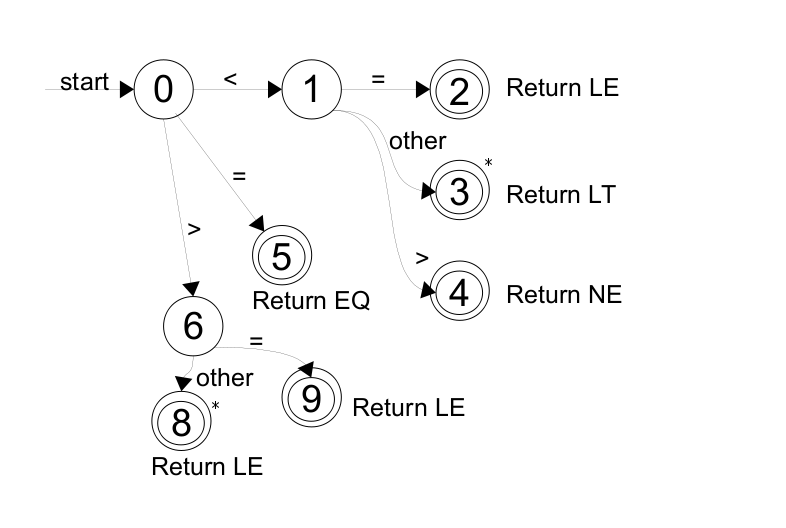
\includegraphics[scale=0.50]{snapshot1.png}
\else
%	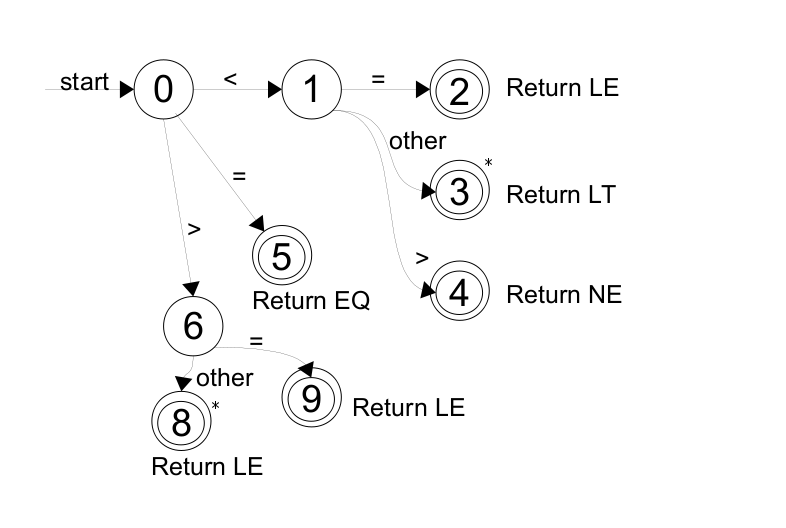
\includegraphics[scale=0.50]{snapshot1.png}
\fi
\caption{Transition diagram for relational operators.}
\label{fig:1}
\end{center}
\end{figure}

\begin{figure}[htb]
\begin{center}
\ifpdf
	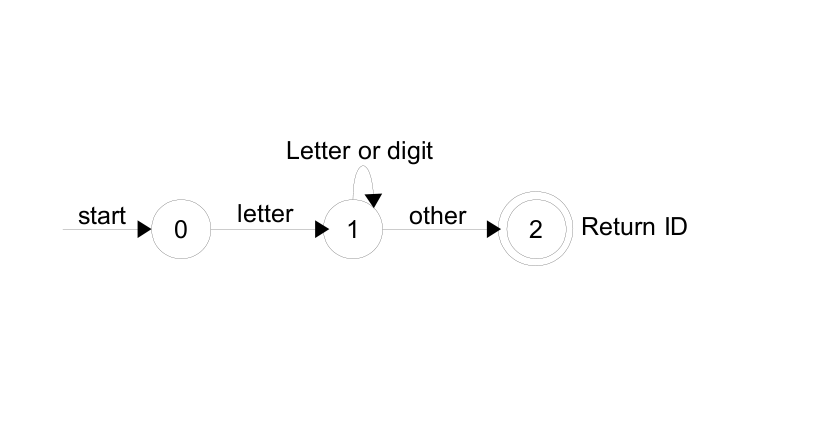
\includegraphics[scale=0.50]{snapshot3.png}
\else
%	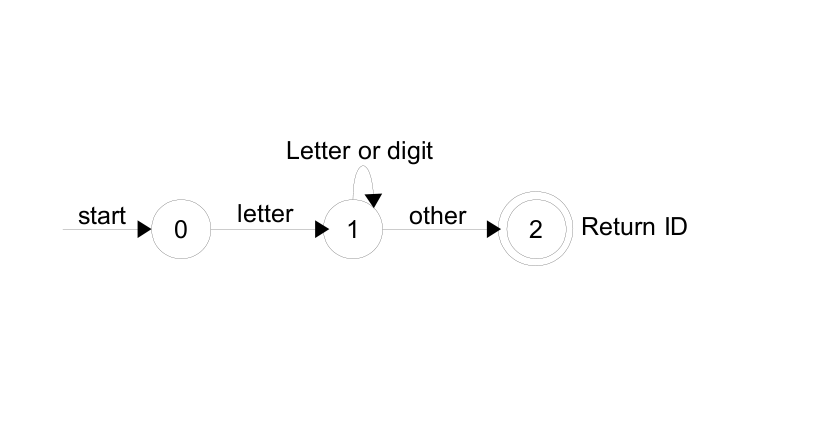
\includegraphics[scale=0.50]{snapshot3.png}
\fi
\caption{Transition diagram for recognising identifiers.}
\label{fig:2}
\end{center}
\end{figure}

\subsection{Transition diagram for reserved words and identifiers}
\paragraph{}
keywords like \emph{if} or \emph{then} are reserved, so they are not identifiers even though they look like identifiers.To recognise the identifier the transition diagram as shown in fig:2.



\subsubsection{Steps to follow to recognise keywords}

\begin{itemize}
\item Install the reserved word in symbol table initially.

\item Create separate transition diagram for each keywords.

\end{itemize}

\subsection{Transition diagram for unsigned number}
Transition diagram for token \emph{number} is as shown in Figure 3. 



\begin{figure}[htb]
\begin{center}
\ifpdf
	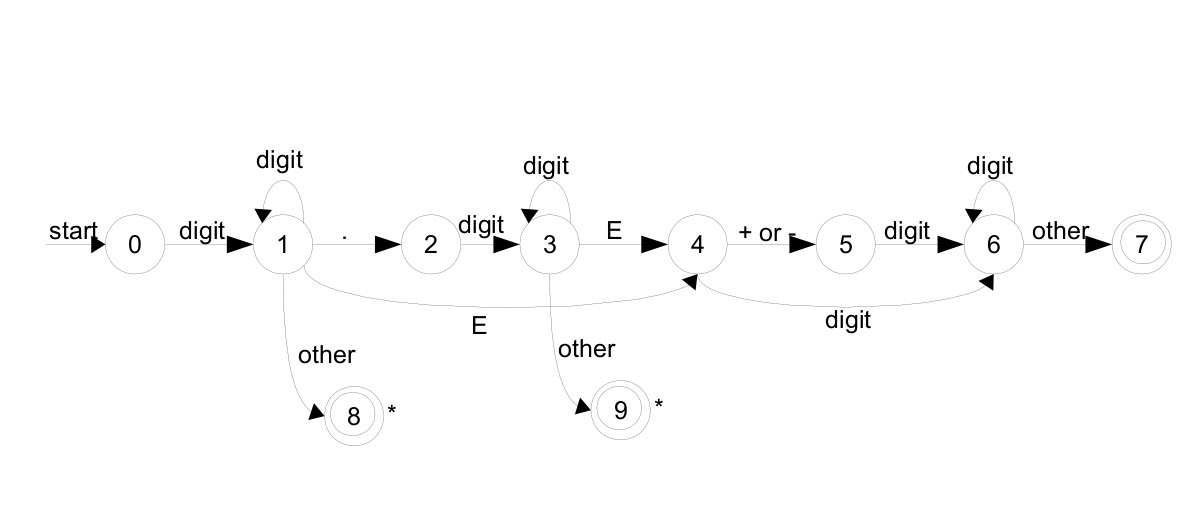
\includegraphics[scale=0.40]{snapshot2.png}
\else
%	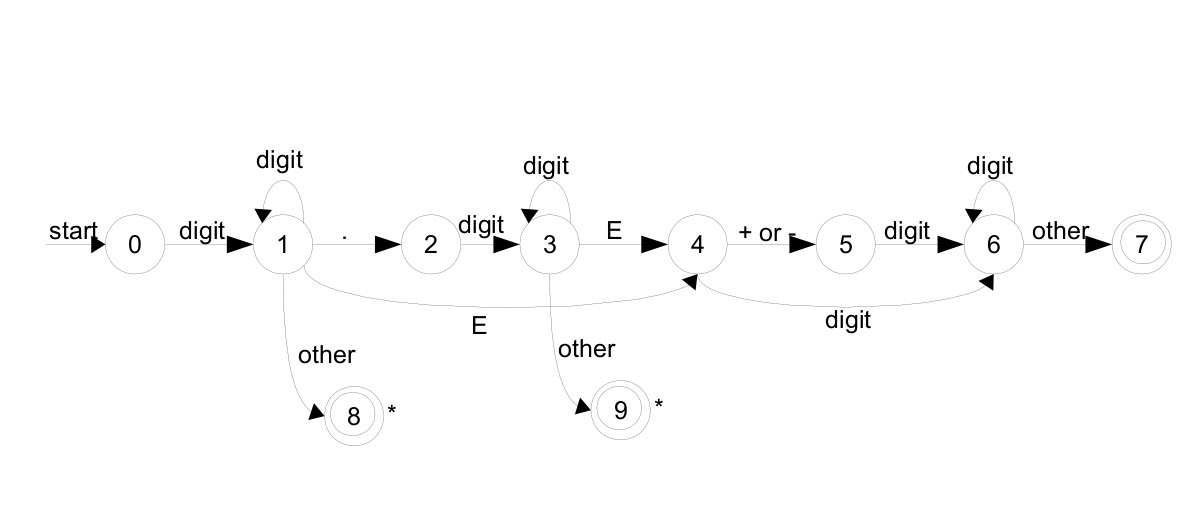
\includegraphics[scale=0.40]{snapshot2.png}
\fi
\caption{Transition diagram for unsigned number.}
\label{fig:3}
\end{center}
\end{figure}


\section{Grammar of our language}
\paragraph{}
Since our language is subset of 'C',the program is collection of blocks. Each block may contain one or more statements. The block is opened by the character \{ and the block terminates by \}. The production is as shown below.

\begin{tabular}{ccc}
%% row 1
&
&
\\
\emph{program}
&$\rightarrow$
&\emph{block}
\\
%% row 2
\emph{block}
&$\rightarrow$
&'\{' \emph{stmts} '\}'
\\
%% row 3
\emph{stmts}
&$\rightarrow$
&\emph{stmts1} \emph{stmt}
\\
%% row 4

&$\mid$
&$\varepsilon$
\\
&
&
\end{tabular}

\paragraph{}

It is clear that statement has vast option it may start with expression or may \emph{if} statement or it may loop construct. All this options are grouped in \emph{FIRST(stmt)}. Let us look at productions of \emph{stmt}.

\begin{tabular}{ccc}
%% row 1
&
&
\\
\emph{stmt}
&$\rightarrow$
&\emph{expr} ;
\\
%% row 2

&$\mid$
&\emph{IF}
\\
%% row 3

&$\mid$
&\emph{FOR}
\\
%% row 4

&$\mid$
&\emph{block}
\\
&
&

\end{tabular}
\paragraph{}

For the above productions \emph{IF} and \emph{FOR} are still non terminals, they again have the following grammar.

\begin{tabular}{ccc}
%% row 1
&
&
\\
\emph{IF}
&$\rightarrow$
&\textbf{if} ( \emph{expr} ) \emph{stmt1}
\\
%% row 2

&$\mid$
&\textbf{if} ( \emph{expr} ) \emph{stmt1} \textbf{else} \emph{stmt2}
\\
%% row 3
\emph{FOR}
&$\rightarrow$
&\textbf{for} ( \emph{expr1} ; \emph{expr2} ; \emph{expr3} ; ) \{ \emph{stmt}  \}
\\
\end{tabular}

The production of \emph{expr} contains arithmetic expression or relation expression which the language supports.

\begin{tabular}{ccc}
%% row 1
\\
\emph{expr}
&$\rightarrow$
&\emph{rel} = \emph{expr1}
\\
%% row 2

&$\mid$
&\emph{rel}
\\
%% row 3

&
&
\\
%% row 4
\emph{rel}
&$\rightarrow$
&\textbf{id} $<$ \textbf{id}
\\
%% row 5

&$\mid$
&\textbf{id} $<=$ \textbf{id}
\\
%% row 6

&$\mid$
&\textbf{id} $>$ \textbf{id}
\\
%% row 7

&$\mid$
&\textbf{id} $>=$ \textbf{id}
\\
%% row 8

&$\mid$
&\textbf{id} $!=$ \textbf{id}
\\
%% row 9

&$\mid$
&\textbf{id}
\\
%% row 10

&
&
\\
%% row 11
\end{tabular}

For a detailed description of all the grammars used in our language, please refer to the section \emph {Grammars} at last.

\section{Tokens and Symbol Table}
A token is identified by two parts - $<$tokenName, attribute$>$.  TokenName is given by a value as given by the macro definition and it identifies a token type.  Attribute is the lexeme itself.  A token is returned from the lexer everytime a parser is in need of it.

\emph{Symbol table} are data structure that are used by compilers to hold information about source program constructs.  An entry in the symbol table resembles a token.  A set of predefined macros are used for the general constructs of the language.  The symbol table is a linked list that has 2 visible fields.  One is the token ID that specifies what type of lexeme it is storing n the other is the attribute or the lexeme itself.  The last field is a pointer to the next entry of the symbol table.  Our symbol table is divided into two parts:
\begin{itemize}
\item First part consists of the keywords or reserve words of our language.  It also includes all the ASCII symbols and operators. It is initialized at start by a call to installation of keywords.  This part is fixed and unchangeable at all times.
\item Second part consists of all the user defined identifiers.  Insertion of these identifiers into the symbol table starts from IDHEAD.  On arrival of a new lexeme, it is looked up in the symbol table for its entry.  If that particular entry is found, the corresponding token is returned otherwise a new entry in the symbol table is created and token is returned.  During lookup, the entire symbol table needs to be searched and in the case of a new entry traversal is made from IDHEAD.
\end{itemize}

\paragraph{}
Some symbol table entries are as shown bellow. 
\begin{center}


\begin{tabular}{|c|c|}
\hline
%% row 1
\textbf{id}
&\textbf{attribute}
\\\hline
%% row 2
INT
& 260
\\\hline
%% row 3
FL
& 261
\\\hline
%% row 4
CH 
&262
\\\hline
%% row 5
IN 
&268
\\\hline
%% row 6
IF 
&270
\\\hline
%% row 7
EL 
&271
\\\hline
%% row 8
FR 
&275
\\\hline
%% row 9
EQ 
&279
\\\hline
%% row 10
NE 
&280
\\\hline
\end{tabular}
\end{center}

\section{Implementation of \emph{lexer}}
\paragraph{}
The lexer keeps global variables to keep track of its input.  It uses a file pointer, that is initialized to the start of the source program.  A variable `ch' gets the characters from the input stream using the file pointer.  Also the maximum size of the lexeme is fixed to the macro value MAX\_SIZE.  Finally, the value in the macro IDHEAD is used to initialize the symbol table, from which the entries of the identifiers into it starts.\\

The lexer maintains a temporary buffer into which the input stream is written.  It is then checked with the symbol table for any entry in the same name.  If so, the symbol table returns a token from its entry else a new entry is made and that token is returned.  The buffer is discarded at the time of returning the token to the parser.\\

The following comparisions are done for getting the lexemes:
\begin {itemize}
\item First a check is made for the whitespaces.  If any whitespace is found it is suitably discarded and the lexer starts scanning its next input.  Only in the case of a newline, the lexer increments the global newline count by one.

\item If the current character (ch) is a delimiter, then it is checked for the comments and relational operators.  The automata described above for relational operators is used.  A lookahead character (lach) is kept that points one character ahead of the current character.  The following situations may arise depending on the contents of `ch' and `lach':\\

\begin {itemize}
\item If ch = `/' and lach `=' *:  It indicates the existence of a comment.  Therefore, the comment continues till `*/' and hence everything scanned is discarded until ch = `*' and lach = `/'.

\item if ch = `=' and lach = `=': A token for the relational operator `==' is returned to the parser.
\item if ch = `$<$' and lach = `=': A token for the relational operator `$<$=' is returned to the parser.  If lach is anything other than `=', then a token for the relational operator `$<$' is returned to the parser and one character from input stream, that is, lach is retracted back as per the automata (denoted by a * in automata for retraction).
\item if ch = `$>$' and lach = `=': A token for the relational operator `$>$=' is returned to the parser.  If lach is anything other than `=', then a token for the relational operator `$>$' is returned to the parser and lach is retracted back as per the automata.
\item if ch = `!' and lach = `=': A token for the relational operator `!=' is returned to the parser.
\end {itemize}

\item The character is now checked for the existence of any of the operators (+, -, *, /, $\{$, $\}$, $($, $)$, ;, , , =) and a token corresponding to the operator is retracted back.

\item The lexer now for numbers as per the automata of numbers.  If the current character is within 0-9, a flag is set saying it as an integer number.  Successive numbers are entered into a buffer.  If the current character becomes `.', and if next character is a digit, then it is a float number and the flag is set to float.  Successive numbers are entered into the buffer.  But if the next character is not a digit, then its an error and lexing is continued from first.  Also, if the current character is not a `.' and not a delimiter, then it is an error.  Finally, if no error occurs, a token is returned to the parser, depending on the flag value.

\item The lexer checks for identifiers.  If the current character is within a-z or A-Z and not a digit, then it is the start of an identifier.  A new character is scanned everytime and filled into a buffer until the new character is not a delimiter.  If the current character is `.', then it is an error, as no dots can appear in an identifier of a C subset language.  Finally, a pointer is retracted.  The identifier is checked in the symbol table for its entry.  If there is no entry in the symbol table, a new entry is made and a token for the identifier is returned to the parser otherwise a token from the existing symbol table entry is returned to the parser.
\end {itemize}

\section{Implementation of \emph{Parser}}
\paragraph{}
The parser uses the first components of the tokens produced by the lexical analyzer to create the tree like intermediate representation that depicts the grammatical structure if the token stream.  A recursive descent top-down parsing technique is followed to parse the input.


The function \emph{void match (char *string)} matches the parameter with the next lexeme. If it does not match, an explicit error handling is done by printing the required `string' from the grammar.

The parser consists of a global lookahead token.  It is initialised at start by a call to lexer, that returns a token.  Further updations of the lookahead token is done in the call to `match', where the current lexeme expected from the grammar is checked with the lexeme in the input string, that is held in the lookahead token.  After a successful match, the lookahead is updated with a new token by a call to the lexer.  This process continues till the end of file is reached.

A grammar like\\
\hspace{1.5in} A $\rightarrow$ aB\\
\hspace{1.5in} B $\rightarrow$ b\\
is implemented using function call for each of the non-terminals.  The terminals defined in the FIRST ($\alpha$), like FIRST (A) = {a}, guide the parsing actions, that is, depending on the current terminal symbol in the FIRST ($\alpha$) leads to different paths or productions during parsing.  The above grammar is implemented from the start function S as,\\
S ()\\
$\{$\\
\hspace{.5in} A (); /* A function call to non-terminal A */\\
$\}$\\\\
A ()\\
$\{$\\
\hspace{.5in} match ("a"); /* A match is made for the terminal `a' */\\
\hspace{.5in} B (); /* A function call to non-terminal B */\\
$\}$\\\\
B ()\\
$\{$\\
\hspace{.5in} match ("b"); /* A similar match for terminal 'b' */\\
$\}$\\

This implementation results in an infinite recursion if the grammar is left recursive, that is a production calling its own production at start like A $\rightarrow$ AB results in an infinite recursion.  Also if two or more productions have the same starting terminals, then it needs to be factored as the starting terminals or the FIRST ($\alpha$) guides the parsing actions. Therefore, grammars that are implemented should be left recursion eliminated and left factored.  Such an implementation is done during our parsing and the grammar used is shown in the section of \emph {Grammars} at last.

Finally, a parse tree is generated alongwith parsing by constructing tree nodes explicitly while the `match' is done for a lexeme.

\section{Example program}
\paragraph{}
 
 Consider the example program \emph{test1.cs}.
 \begin{figure}[htb]
 \begin{center}
 \ifpdf
 	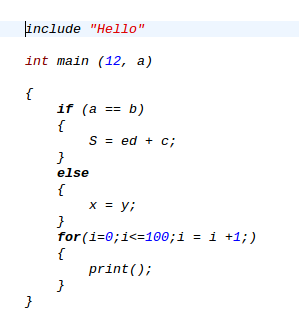
\includegraphics[scale=0.750]{snapshot4.png}
 \else
 %	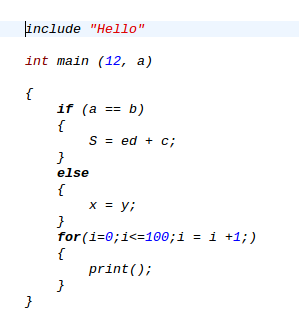
\includegraphics[scale=0.750]{snapshot4.png}
 \fi
 \caption{Example program}
 \label{fig:4}
 \end{center}
 \end{figure}
\paragraph{}
The above program involves both \emph{if-else} and \emph{for-loop} constructs. Where \emph{int main()} considered as a function.
We have \emph{Makefile} to create \textbf{a.out}.After executing \emph{make} we can call a.out with program as the parameter.
\begin{figure}[htb]
\begin{center}
\ifpdf
	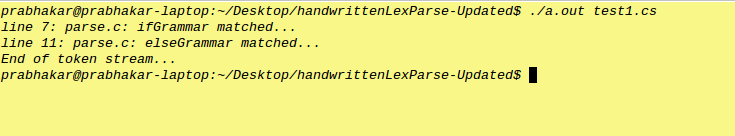
\includegraphics[scale=0.81]{snapshot5.png}
\else
%	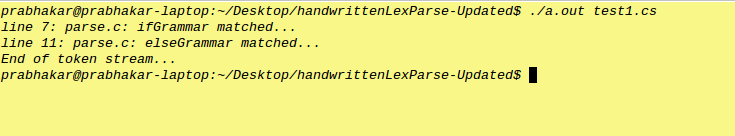
\includegraphics[scale=0.81]{snapshot5.png}
\fi
\caption{Output on the terminal after parsing.}
\end{center}
\end{figure}


\paragraph{}
Once \emph{a.out} is executed the file \emph{dotty.dot} is created which can be used as input to \emph{dotty} or \emph{kgraphviewer} to view the explicit parse tree. The parse tree for the \emph{test1.cs} is as shown below.
\begin{figure}[htb]
\begin{center}
\ifpdf
	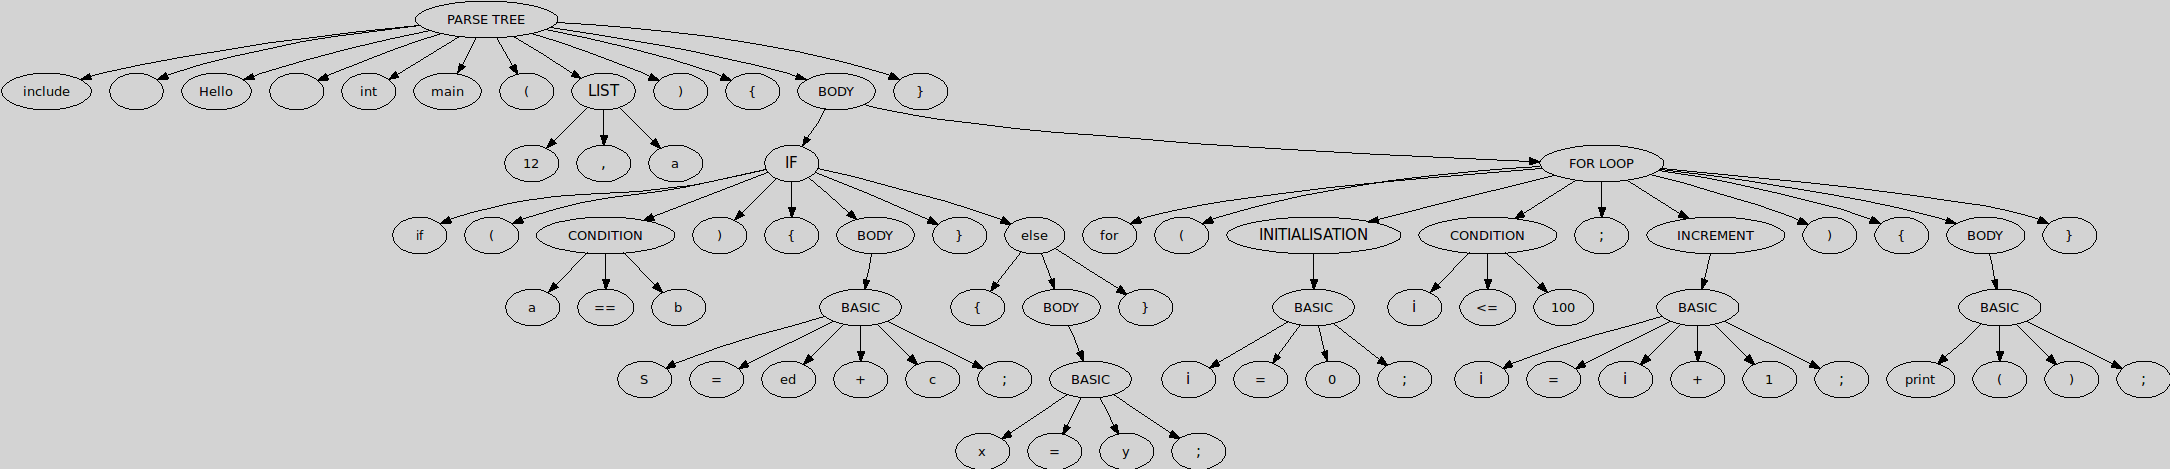
\includegraphics[scale=0.3]{parsetree.png}
\else
%	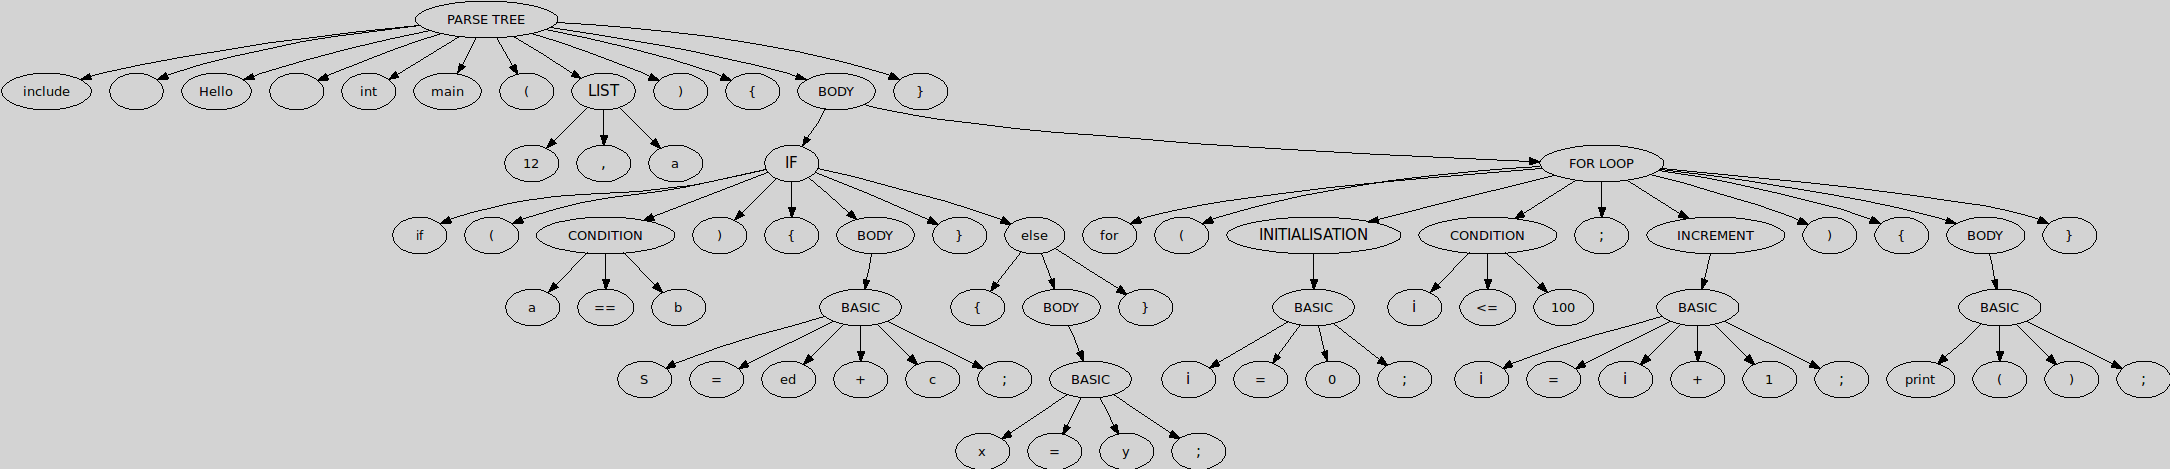
\includegraphics[scale=0.54]{parsetree.png}
\fi
\caption{Parse tree for the program test1.cs}
\end{center}
\end{figure}

\section{Parse Tree}

The parse tree pictorially shows how the start symbol of the grammar derives a string in the language. A typical parse tree for our language is as given in the figure of typical Parse Tree.
\begin{figure}[htb]
\begin{center}
\ifpdf
	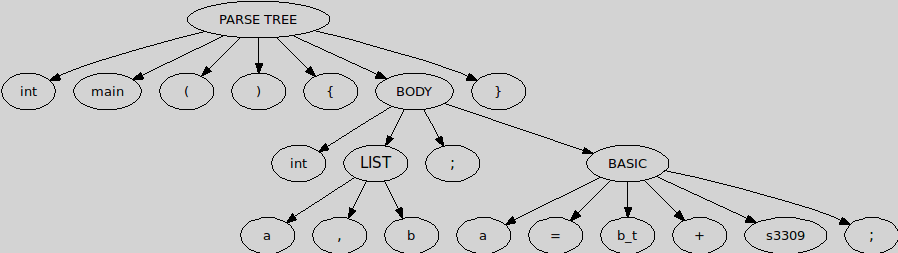
\includegraphics[scale=0.60]{simple.png}
\else
%	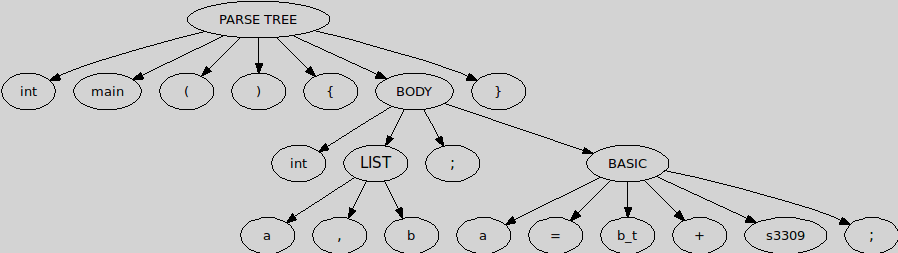
\includegraphics[scale=0.60]{simple.png}
\fi
\caption{Typical Parse Tree.}
\end{center}
\end{figure}

\section{Grammars}
The following are the left recursion eliminated, left factored grammars used in the implementation.  The first production is the program start.  All productions are self explanatory and all non-terminals are capitalized.\\\\
S :

\hspace{.25in} PROGRAM\\\\
PROGRAM :

\hspace{.25in} INCLUDE FUNCTIONS\\\\
INCLUDE :

\hspace{.25in} include "IDENTIFIER" INCLUDE $|$ $\epsilon$\\\\
FUNCTIONS :

\hspace{.25in} KEYWORD IDENTIFIER $($LIST$)$ BODY FUNCTIONS $|$ $\epsilon$\\\\
BODY :

\hspace{.25in} $\{$ STATEMENT $\}$ BODY $|$ $\epsilon$\\\\
DECLARATION :

\hspace{.25in} KEYWORD LIST ; DECLARATION $|$ $\epsilon$\\\\
STATEMENT  :

\hspace{.25in} IF $|$ FOR $|$ STATEMENT'\\\\
STATEMENT' :

\hspace{.25in} BASICSTATEMENT $|$ $\epsilon$\\\\
FOR :

\hspace{.25in} for $($BASICSTATEMENT; CONDITION; BASICSTATEMENT$)$ BODY\\\\
IF   :

\hspace{.25in} if CONDITION BODY ELSE\\
ELSE :

\hspace{.25in} else BODY\\\\
BASICSTATEMENT :

\hspace{.25in} IDENTIFIER = EXPR ; BASICSTATEMENT

\hspace{.25in} $|$ IDENTIFIER $($LIST$)$ ; BASICSTATEMENT $|$ $\epsilon$ $|$ ;\\\\
CONDITION :

\hspace{.25in} IDENTIFIER RELCOND IDENTIFIER\\\\
KEYWORD :

\hspace{.25in} int $|$ float $|$ char $|$ $\epsilon$\\\\
LIST    :

\hspace{.25in} IDENTIFIER SUBLIST $|$ $\epsilon$\\
SUBLIST :

\hspace{.25in} , IDENTIFIER SUBLIST $|$ $\epsilon$\\\\
EXPR :

\hspace {.25in} TERM SUBEXPR\\
SUBEXPR :

\hspace {.25in} + TERM SUBEXPR $|$ - TERM SUBEXPR $|$ $\epsilon$\\
TERM :

\hspace {.25in} FACTOR SUBTERM\\
SUBTERM :

\hspace {.25in} * FACTOR SUBTERM $|$ / FACTOR SUBTERM $|$ $\epsilon$\\
FACTOR :

\hspace {.25in} $($ EXPR $)$ $|$ IDENTIFIER\\

RELCOND :

\hspace{.25in} IDENTIFIER $<$ IDENTIFIER

\hspace{.25in} $|$ IDENTIFIER $<$= IDENTIFIER

\hspace{.25in} $|$ IDENTIFIER $>$ IDENTIFIER

\hspace{.25in} $|$ IDENTIFIER $>$= IDENTIFIER

\hspace{.25in} $|$ IDENTIFIER == IDENTIFIER

\hspace{.25in} $|$ IDENTIFIER != IDENTIFIER

\hspace{.25in} $|$ IDENTIFIER\\\\
IDENTIFIER :

\hspace{.25in} id\\\\

\section{References}
\begin{itemize}
\item Lex and Yacc by John R. Levine, Tony Mason, Doug Brown - O’Reilly Publications
\item A Compact Guide to Lex and Yacc by Tom Niemann at \href{http://epaperpress.com}{epaperpress.com}
\item Compilers Principles Techniques and Tools by Afred V.Aho, Monica S.lam, Ravi Sethi,Jeffrey D.Ullman
\item \href{http://en.wikipaedia.org/wiki/Syntax analysis}{Wikipaedia}
\end{itemize}


\end{document}